\documentclass[a4paper, 12pt]{report}
\usepackage[a4paper, top=2cm , bottom=2cm , right=2cm , left=2cm ]{geometry}

\usepackage{graphicx} % Required for inserting images
\usepackage[T1]{fontenc}
\usepackage[english]{babel}
\usepackage[utf8]{inputenc}
\usepackage{titlesec}
\usepackage{xcolor}
\usepackage{amsfonts}
\usepackage{wrapfig}
\usepackage{amssymb}
\usepackage{amsbsy}
\usepackage{float}
\usepackage{soul}
\usepackage[makeroom]{cancel}
\usepackage[framemethod=tikz]{mdframed}
\usepackage{mathtools}
\usepackage{matlab-prettifier}
\usepackage{subcaption}
\usepackage{bm}
\usepackage{tikz}
\usepackage{colortbl} % for cell color in matrices
\usepackage{booktabs}
\usepackage{amsmath}
\usepackage{xcolor}
\usepackage{tcolorbox}
\usepackage{tikz} %for block diagrams
\usepackage{amssymb}

\usetikzlibrary{positioning}

\definecolor{myblue}{RGB}{30, 131, 197}
\definecolor{mygreen}{HTML}{25da18}
\definecolor{myyellow}{RGB}{255, 255, 0}
\definecolor{mygrey}{RGB}{100, 100, 100}
\definecolor{myred}{RGB}{255, 55, 55}

\newtcolorbox{factbox}[1][]{
    colback=mygreen!5,   % Background color
    colframe=mygreen!30, % Frame color
    fonttitle=\bfseries,  % Title font
    title=#1,             % Title
    coltitle = black,   %title color
    sharp corners=southwest,
}
\newtcolorbox{QandAbox}[1][]{
    colback=myred!5,   % Background color
    colframe=myred!20, % Frame color
    fonttitle=\bfseries,  % Title font
    title=#1,             % Title
    coltitle = black,   %title color
    sharp corners=southwest,
}

\newtcolorbox{example}[1][]{
    colback=mygrey!3,   % Background color
    colframe=mygrey!20, % Frame color
    fonttitle=\bfseries,  % Title font
    title=#1,             % Title
    coltitle = black,   %title color
    sharp corners=southwest,
}
% Do not indent paragraphs
\usepackage[parfill]{parskip}

% In case of an image at the bottom, but the footnote below the image (without this the image will be below the footnote)
\usepackage[bottom]{footmisc}

% --------- CUSTOM HEADER ----------
% Modifies the style of the header
\usepackage{fancyhdr}         
\pagestyle{fancy}
\fancyhf{}

% Sets as header: curr_section <space> page_number
\lhead{\rightmark}
\rhead{\textbf{\thepage}}

% Removes the page number at the beginning of chapters
\fancypagestyle{plain}{
  \fancyfoot{}
  \fancyhead{}
  \renewcommand{\headrulewidth}{0pt}
}

% Do not capitalize section name in header
\renewcommand{\sectionmark}[1]{\markright{\thesection.\ #1}{}}

% ------------ NEW ENVS ------------
% ---------- Proof environment ----------
\newenvironment{proof}
{\begin{mdframed}[leftmargin=15pt, rightmargin=15pt, leftline=false, rightline=false] \textit{\underline{Dim.}} \\[10pt] \textit\bgroup}
{\egroup \par \raggedleft $\square$ \end{mdframed}}

% Proof without top and bottom borders
\newenvironment{proof2}
{\vspace*{10pt} \begin{mdframed}[leftmargin=15pt, rightmargin=15pt, leftline=false, rightline=false, bottomline=false, topline=false] \textit{\underline{Dim.}} \\[10pt] \textit\bgroup}
{\egroup \par \raggedleft $\square$ \end{mdframed}}

% ---------- Addendum environment ----------
\newenvironment{addendum}
{\begin{mdframed}[leftmargin=15pt, rightmargin=15pt, leftline=false, rightline=false] \textit\bgroup}
{\egroup\hfill $\diamond$\end{mdframed}}


% ---------- NEW COMMANDS ----------
% ---------- Circled number ----------
\newcommand*\circled[1]{\tikz[baseline=(char.base)]{\node[shape=circle,draw,inner sep=2pt] (char) {#1};}} % 

% ---------- Real numbers and complex numbers shortcuts ----------
\newcommand{\R}{\mathbb{R}}
\newcommand{\C}{\mathbb{C}}




% Make references clickable and change style of links to blue
\usepackage{hyperref}
\hypersetup{
	colorlinks=true,
	linkcolor=blue,
	filecolor=magenta,      
	urlcolor=cyan,
}

\graphicspath{ {images/} }

\titlespacing{\title}{10pt}{50pt}{50pt}
\titlespacing{\chapter}{0pt}{10pt}{10pt}
\titlespacing{\section}{0pt}{35pt}{10pt}

\title{
    \textbf{\Huge{Laboratory of Robust Identification and Control}}\\
    \textit{Lecture notes}
}
\author{A. Ayanmanesh Motlaghmofrad}
\date{A.Y. 2024/2025}


% Force all math to use \displaystyle by default
\everymath{\displaystyle}

\linespread{1.2} % Adjusts line spacing to 1.5

\begin{document}
\maketitle
\tableofcontents


% ---------------------------------------------------------------------
% ------------------------ MODIFY ONLY BELOW --------------------------
% ---------------------------------------------------------------------
% ---------------------------------------------------------------------

\chapter{Introduction}    % For a new chapter (works in book and report class)
\subsubsection{Disturbances and uncertainties}
% page1
% -------------------------------------

    The key word \textit{Robust} suggests that we are taking uncertainties into account. The model of the plant is as following:

%Graph
\begin{figure}[htbp]
    \centering
    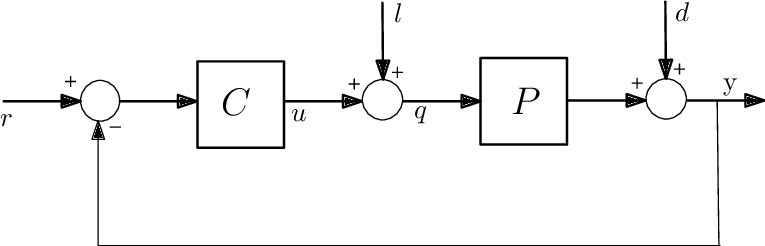
\includegraphics[width=\textwidth]{images/1.png} % Adjust width as needed
    \caption{A general control plant with additive disturbances \textit{l} and \textit{d}}
    \label{fig:graph_label}
\end{figure}


The general nonlinear state-space representation of the system is:

\begin{equation}
    \begin{cases}
    \dot{x}(t) = f(x(t), u(t)) \\
    y(t) = g(x(t), u(t))
    \end{cases}
\end{equation}
Where:
\begin{itemize}
    \item $x(t)$ is the state vector,
    \item $u(t)$ is the input vector,
    \item $y(t)$ is the output vector,
    \item $f(\cdot)$ is a nonlinear function describing the system dynamics,
    \item $g(\cdot)$ is a nonlinear function describing the output equation.\\
\end{itemize}

%page 2
%--------------------------------------------------
    \textbf{The first step} of any control problem is typically \textbf{derivation of mathematical model of the plant.} This step is the most crucial step, because if we drive the model by applying first principles of physics, we are likely to adopt approximated models, adopting simplifying assumptions, e.g. rigid body assumption etc. Further, the value of the physical parameters involved in the equations, such as friction coefficient, are not exactly known. Such approximations introduce errors and uncertainty in the mathematical description of the plant to be studied and controlled.

% page 3
% -----------------------------------------------------
    This fact is critical, since standard approaches to controller design are model-based; that is, the controller design has a strong dependency on the mathematical models used to describe the plant to be studied and controlled.


\begin{center}
$\textit{\textbf{Neglecting some physical details}} \equiv \textit{\textbf{Neglecting some state variables}}$
\end{center}

    For example, for modelling a robotic arm, generally, rigidity is assumed for the joints. Nevertheless, in fast movements  this assumption does not hold anymore, and the model does not predict the real performance of the robot, neglecting some state variables. Further, in some applications, we are not even aware of the phenomenon or phenomena that is being neglected. 

\subsubsection{Counter act for disturbances and uncertainties}

\begin{itemize}
    \item \textbf{First counter act}  These uncertainties and disturbances directly affect the controller design in the time domain, since the feedback gain and observer are directly calculated by solving algebraic equations including physical parameters with uncertainties. Nontheless, In frequency domain, the design of the controller is less affected by these uncertainties. 

    This does not mean that \textit{Transfer Function} is not affected by uncertainties of the parameters, because not considering some phenomona leads to the transfer function having less poles or zeros and because the uncertainty of the parameters affect the coefficients of the complex variables, being \textit{s} or \textit{z}. In the frequency domain design, we design the controller based on the frequency response of the system, considering cutting frequencies that reject high-frequency and low-frequency disturbances. In addition, by considering phase-margin and gain-margin, some margin for disturbances and uncertainties are taken into accoutn.

\textbf{Question to be answered: the sensitivity function is high-pass filter, meaning that the high frequency phenomenon, on the other-hand T is a low-pass filter, if the plant is designed for having a fast rising time, high-frequency phenomena also passes T.}

    \item \textbf{Second counter act}: Optimization problems in state-space where introduced to tackle this problem.
    \item \textbf{Third counter act}: Optimization problem, in state space, is combined with the concept of robustness, in frequency space, which is called $H_{\infty}$. 
\end{itemize}


\subsubsection{What is going to be discussed in this course}
    In the first part of this course, we are going to learn how to learn from the mapping from the input to the output of the system, extracting a \textbf{mathematical model} for the plant. Further, it elaborates on this data to drive also a \textbf{discription for uncertainty}. These, together, can be used for \textbf{robust controller design} in a model-based approach.

    In the second step, the aim is to design a controller directly from the data, without the intervention of the model.


\begin{factbox}[Professor's Quote]

    In conclusion, even if the physical model is very precise, at some point, in order to measure the parameters used in the physical models, it is required to do some experimental measurements, subjected to noise, introducing uncertainties to our model.\newline \newline
    If these uncertainties are not taken into account, the controller will not have a good performance when implemented physically, and it is going to work only in simulations. \newline \newline
    There are many approaches to tackle this problem. Here, in the first part of the course, we will focus on \textbf{System Identification}, which is another modelling paradigm. In this paradigm, we learn the mathematical model of the system to be controlled by using experimentally collected data. Not only do we introduce what \textit{System identification} is and what are the possible approached, but maintly to focus on \textbf{\textit{Set-membership Identification Technique}} that allow us to learn the model of the system, and drive information about how the uncertainty is affecting out model; this is used to design a controller in a robust manner. Robust controller designed can be directly applied to the real physical plants.  \newline \newline
    
    In the second part of the course, we shift our paradigm again. In this part, assuming that the collected data represents the behavior of the mapping between the input and output, we try to design the controller directly from the data, called  \textbf{Direct Data-Driver Controller Design}. \newline \newline
    
\end{factbox}

\textit{System identification} deals with the problem of building mathematical model of dynamical systems from sets of experimentally collected input, output data.


\begin{figure}[htbp]
    \centering
    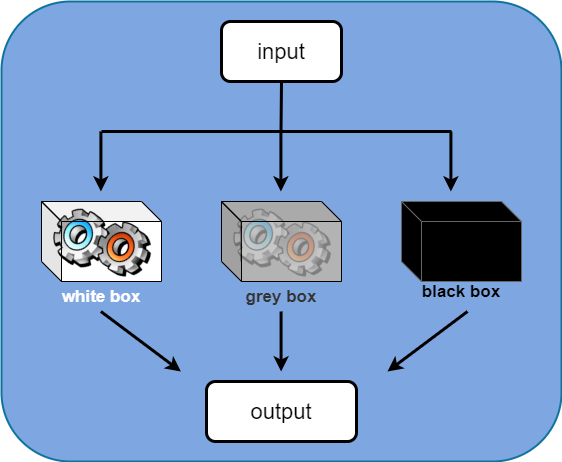
\includegraphics[width=0.5\textwidth]{images/system-id-scheme.png}
    % Adjust width as needed
    \caption{Classifications of System Identification Problems}
    \label{fig:id_classes}
\end{figure}

There are three different approaches to mathematically model dynamical systems:
\begin{enumerate}

\item \textbf{White-box modelling}:\newline Models, in this approach, are obtained by applying \textbf{first principles for physics}. All the physical phenomena and also all the physical parameters involved in the equiation are assumed to be exactly know. This approach was applied in the course of \textit{Automatic Control} for modelling systems.

\item \textbf{Grey-box modelling}: Here, \textbf{models} are base on the equations obtained by applying first principles of \textbf{physics}, but \textbf{the parameters} entering the equations are not completely known, so they need \textbf{to be estimated} from experimental data. 

\item \textbf{Black-box modelling}: In this case, the structure of the equations is selected by the user on the basis of some \textbf{"general" a-priori information}, e.g. linearity, on the system physics, or at any rate by the system properties. \newline 

\begin{factbox}[Professor's Quote]
    In this method, the designer of the system model, has some degree of freedom in selecteing the structure of the model, provided that the model embeds the "general" a-priori information.\newline \newline
    If we do not have any a-priori information, an artificial-neural-network may be selected as the structure of the model.
\end{factbox}
the parameters involved in the equations of the black-box models are \textbf{to be estimated}, or computed, by using experimentally collected data. In general, \textbf{the parameters of a black-box model do not have a clear physical meaning}.
\end{enumerate}


In general, \textbf{white-box models are not very useful in practice}, at least for control applications, because they are based on the assumption that the physics involved in the system under study is well-known.

\subsubsection{The comparison between the grey-box and Black-box models:}
\textbf{Similarity} 
In both cases:
\begin{itemize}
\item physical insight is exploited to drive/select the structure of the equations.
\item experimentally collected data is used to estimate/compute the parameters involved in the equations.
\end{itemize}

\textbf{Difference} 
\begin{itemize}
\item In grey-box modelling, the structure of the equations is not selected by the user, since it is forced by the first principles of physics. This suggests that, in general, the equations of a grey-box model depends, in a possibly complex, non-linear ways, on the physical parameters to-be-estimated.\newline
for instance of a grey-box model:
$\begin{cases}
    \dot{x}(t) = A x(t) + B u(t) \\
    y(t) = C x(t) + D u(t)
\end{cases}$ where:
\newline
\[
A = \begin{bmatrix}
\frac{m}{k^2} & \sqrt{\beta}\\
\frac{\alpha^2.k^3}{\gamma} & 1  
\end{bmatrix}, \quad
B = \begin{bmatrix}
b_1 \\
b_2
\end{bmatrix}, \quad
C = \begin{bmatrix}
c_1 & c_2
\end{bmatrix}, \quad
D = \begin{bmatrix}
d
\end{bmatrix}
\]
In this case, using the physical principles for modelling seems like a good idea; the system is simple, and its physics is well-known. The problem is that the parameters are to-be-estimated. This problem leads to an optimization problem. Now, A difficulty may arise, because if the equation we are going to write so that they relates input and output data obtained experimentally depends on parameters in a complex and non-linear fashion, the mathematical problem of driving what are the correct value of the system parameter satisfying the relation between the intput and output is going to be a complex problem. \textbf{This is the main limitation of grey-box model.}

\item In the black-box version of the same problem, just some general information such as liniearity and time-invariantion is exploited. Now, we found the four matricies \textit{A, B, C, D} in a form that is much simpller, just 4 parameters for A, and so on, for instance. In this case, the system output depends on the input in a way simpler manner.
\[
A = \begin{bmatrix}
a_{11} & a_{12} \\
a_{21} & a_{22}  
\end{bmatrix}, \quad
B = \begin{bmatrix} 
b_1 \\
b_2
\end{bmatrix}, \quad
C = \begin{bmatrix}
c_1 & c_2
\end{bmatrix}, \quad
D = \begin{bmatrix}
d
\end{bmatrix}
\]\newline


\begin{factbox}[Professor's Quote]
    Therefore, in black-box model, we have more freedom to select the struture of the equations in a way that is computationally more convenient, by embedding/exploiting some general properties drived from our physical insight. 
The idea is to consider only the most important a-priori information and/or the information that we trust the most!
\end{factbox}

\end{itemize}

\subsubsection{General procedure for building a grey/black-box modelling:}
Let's compare grey-box and black-box models from the point of view of the parameter estimation problem. While building the mathematical model of the system, in general, we follow a procedure similar to the following one, it be a grey-box or black-box structure:\newline

\begin{enumerate}
    \item to exploint availabe a-priori information on the system under study to select \textbf{the structure of the mathematical equation} describing the input-output mapping.
    \begin{factbox}[Professor's Quote]
The model is always in the input/output form. Signals that we can apply to the system is called input, and signals that we can measure, is called output. If we are in the case where we can measure all \textbf{state variables} involved in the system, we can have a full description of the system. However, in a general case, the system involves input, output, and state variables, but we are able to measure only a subset of physical variables in the system - being the value to be monitored or the control output.

Now, these parameters have physical meaning in grey-box case, or are merely mathematical parameters in black-bock case.
\end{factbox}

In the end of this step, we have a mathematical model of the following form:
\begin{equation}
y(t) = f\left( u(t), \theta\right)
\end{equation}

    \item To collect input-output data representing the behavior of the system under study by performing an experiment. $\tilde{u}$ and $\tilde{y}$ are noise-corrupted data, since, in general, noise can corrupt the output measurements as well as measurement of the input signal applied to the system.
\begin{center}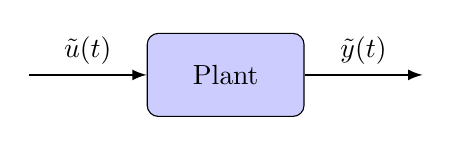
\begin{tikzpicture}[auto, node distance=2.5cm, >=latex]
    % Define styles
    \tikzstyle{block} = [rectangle, draw, fill=blue!20, 
                          text width=5em, text centered, rounded corners, minimum height=3em]
    \tikzstyle{input} = [coordinate]
    \tikzstyle{output} = [coordinate]
    \tikzstyle{arrow} = [thick,->,>=latex]
    
    % Nodes
    \node [input] (input) {};
    \node [block, right of=input] (plant) {Plant};
    \node [output, right of=plant] (output) {};
    
    % Draw arrows
    \draw [arrow] (input) -- node [above] {$\tilde{u}(t)$} (plant);
    \draw [arrow] (plant) -- node [above] {$\tilde{y}(t)$} (output);
\end{tikzpicture}\end{center}
    \item To formulate a suitable mathematical problem to estimate/compute the values of the vector of parameters $\theta$ in such a way that our mathematical model is going to describe the behavior of real system as well as possible.
for example:
\[
\hat{\theta} = \arg \min\limits_{\theta \in S} f(\theta) = \arg \min\limits_{\theta} \|\tilde{y} - f(\tilde{u}, \theta)\|_2
\] 
J(.) here is a \textbf{cost function}. In this case, it is the euclidian norm of $\tilde{y}$ and $f(\tilde{u}, \theta)$.\\
\end{enumerate}
\newpage
At the third stage, the difference between grey-box and black-box models comes into play, since:
\begin{itemize}
    \item In grey-box model: $f(\tilde{u},\theta)$ will, in general depends in a complex, non-linear manner from $\theta$, \textbf{leading to multi-minima convex cost function which is really hard to be minimize}\\ \\
    While\\
    \item In black-box model: $f(\tilde{u},\theta)$ will be selected by the user in order to depend linearly from $\theta$,if possible, or in the simplest possible way, \textbf{leading to a single-minima convex funciton to be minimized}, which is much easier in comparison. \\
\end{itemize}
For example, consider the following multi-minima cost-function: \\

\(
J(\theta_1, \theta_2) = \sin(\theta_1) \cdot \cos(\theta_2) + \frac{\theta_1^2 + \theta_2^2}{10}
\)

\begin{figure}[htbp]
    \centering
    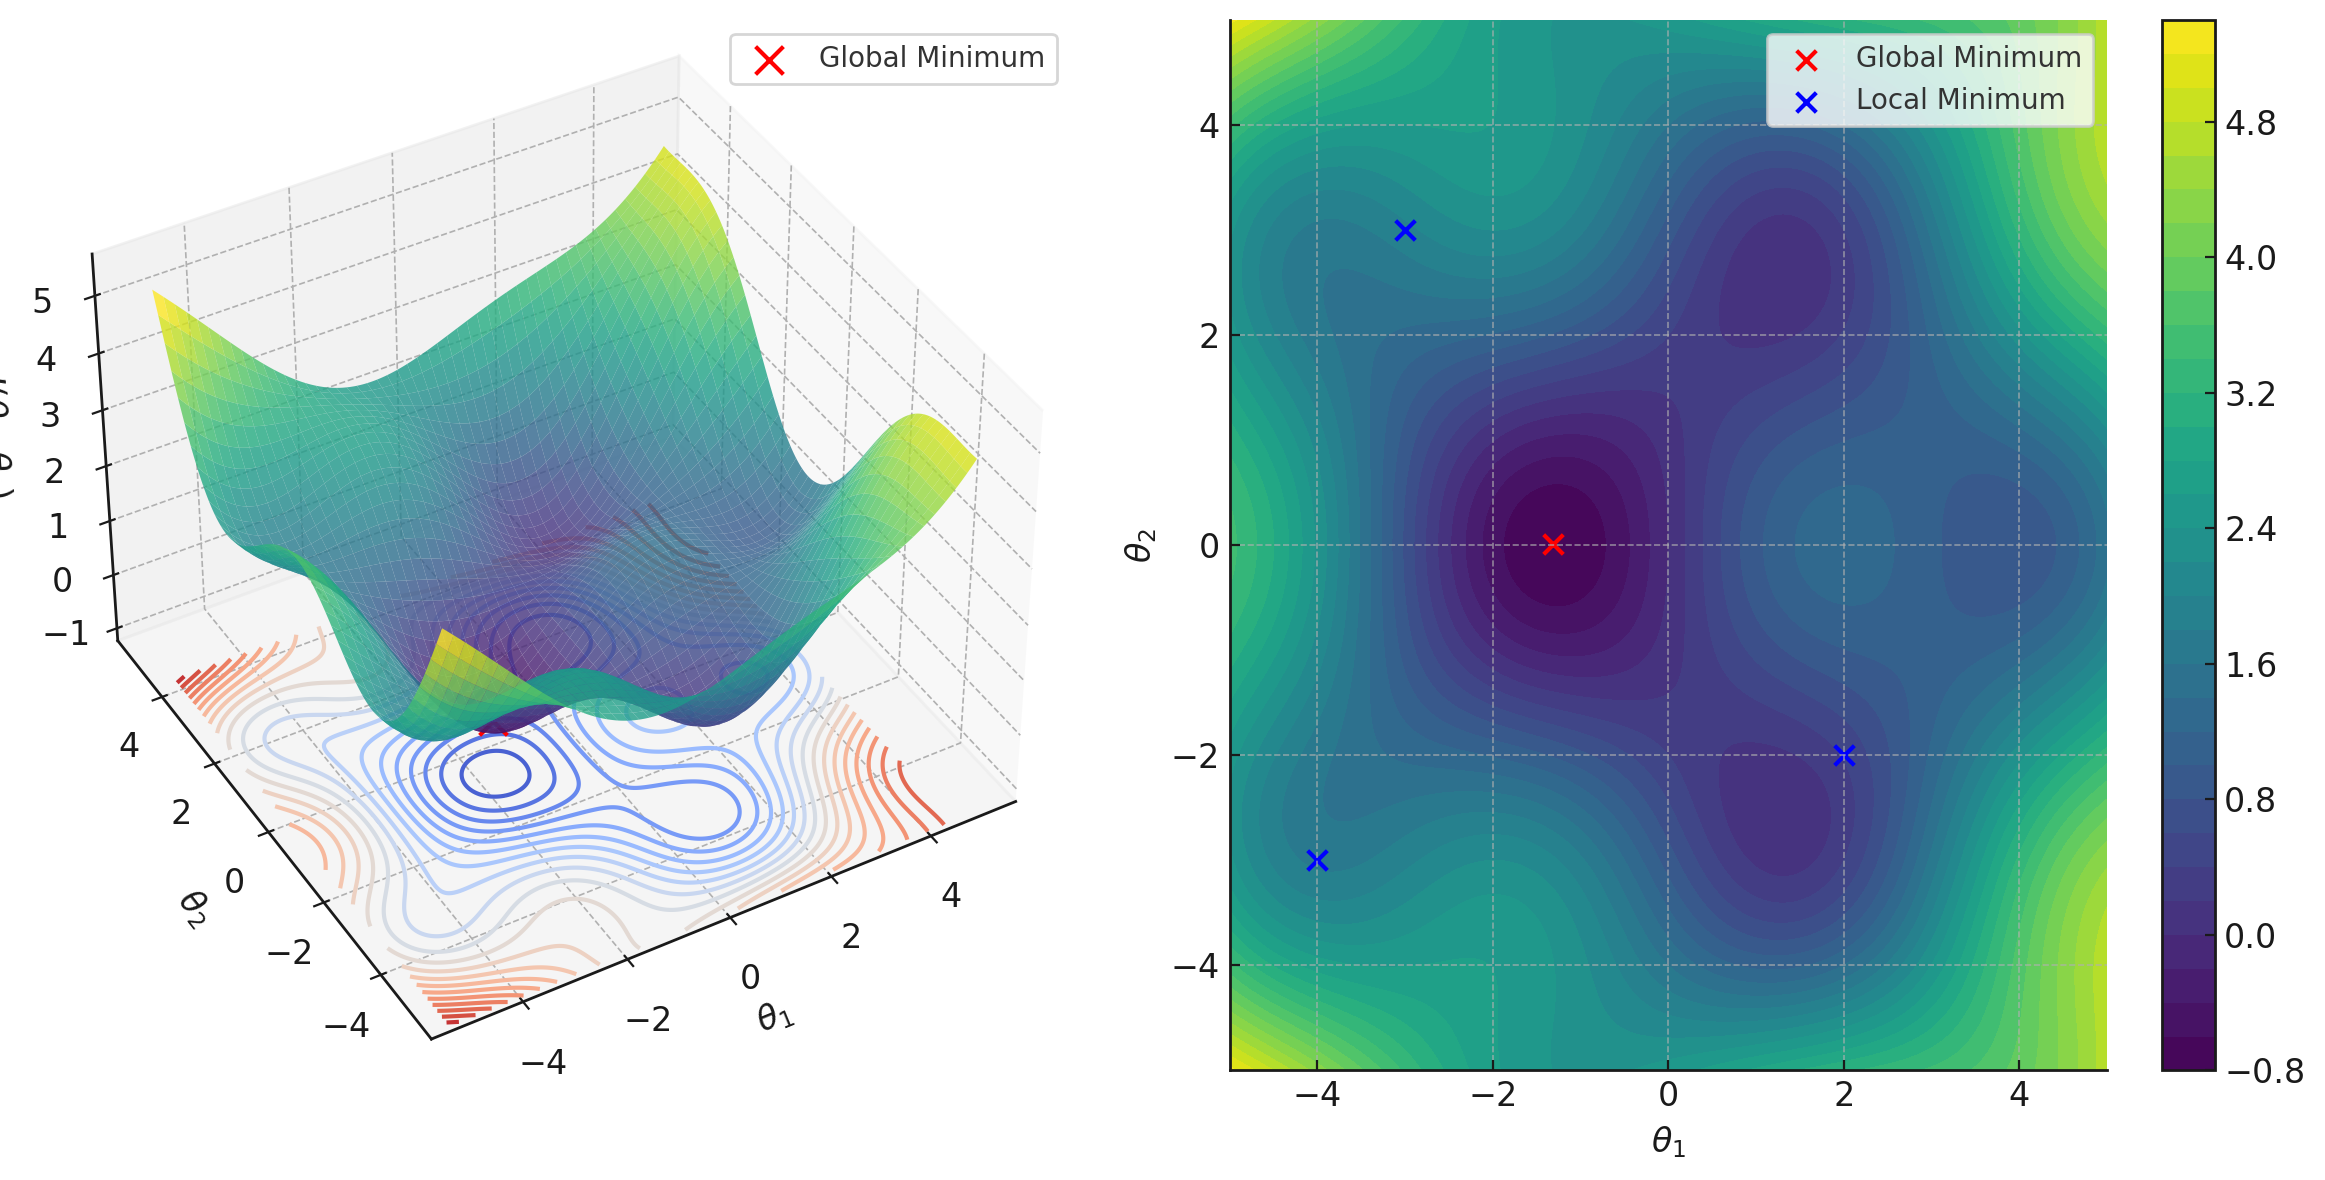
\includegraphics[width=0.75\textwidth]{images/multi-minima-cost-function.png}
    % Adjust width as needed
    \caption{The 3D plot and countor plot of the afforementioned cost-function, which is a multi-minima cost-function}
    \label{fig:multi-minima-cost-function}
\end{figure}

In this example, we look for the global minimum of the cost-function. Finding this point, however, is not an easy task, due to the fact that there is no guarantee that our optimization algorithm will not be trapped in one of the local minima, which may correspond to a "very bad" estimation of $\theta$. Even if we find the global minimum by chance, there is no guarantee that output is indeed the global minima.

On the other hand, When a black-box model is considered, a parametrization is considered so that the function $f(u,\theta)$ is a convex function of $\theta$, thereby having a single global minimum. In this case, no matter what optimization algorithm is used, reaching the global minimum is guaranteed.This is evident in the following cost-function:\\

\(
J(\theta_1, \theta_2) = \theta_1^2 + \theta_2^2
\)
    
\begin{figure}[htbp]
    \centering
    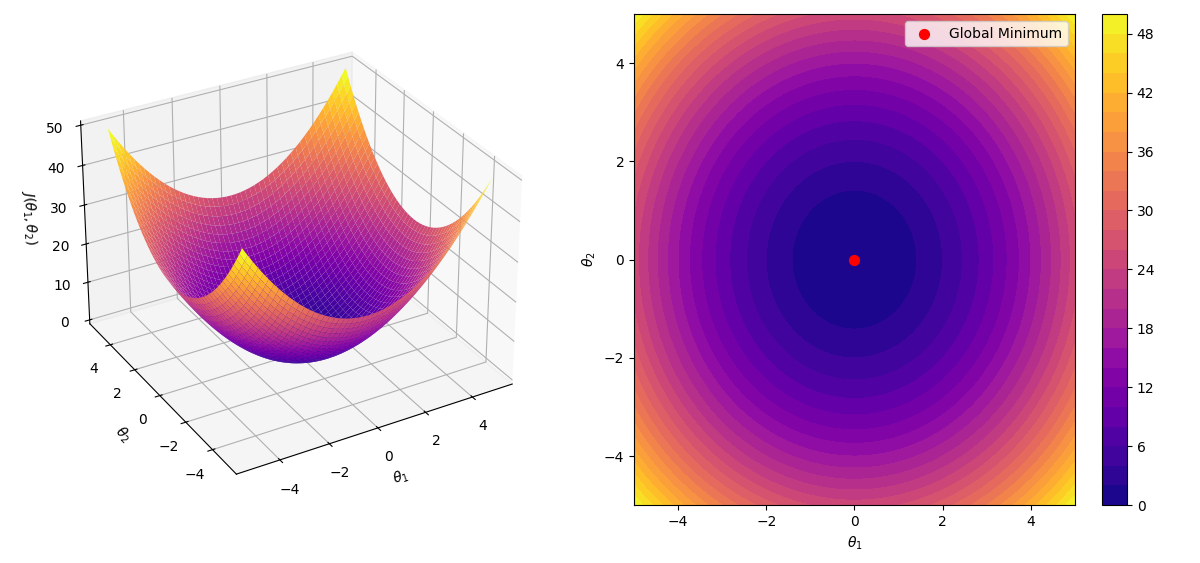
\includegraphics[width=0.75\textwidth]{images/convex-cost-function.png}
    % Adjust width as needed
    \caption{The 3D plot and countor plot of the afforementioned cost-function, which is a convex cost-function}
    \label{fig:multi-minima-cost-function}
\end{figure}


\begin{QandAbox}[Q and A]
    \textbf{Question:} we use grey-box model when we have an insight about the system and parameters. Hence, when we run the optimization problem, we can initialize the optimization problem with more suitable initial condition. Further, we can neglect some of the estimation, knowing that the estimated value does not correspond to the physical quantity the parameter is expected to have.\\
    
    \textbf{Professor's answer:} This is true for simple systems. Nonetheless, in such compolex systems as chemical processes or optical lazer systems, it's hard to have an insight before hand about some parameters. In addition, since we are dealling with multi-dimensional problems, it might be the case that we confine the expected value for some parameters but still, for some parameters, we need to deal with the issue mentioned about the multi-minima cost functions. However, it might be the case that the estimation of those physical parameters are of interest, which is not the concern of this course. Here, we do system identification for control purposees. \\
    
\end{QandAbox}

To clarify the matter further, consider an \textbf{\textit{LTI system}} such that the \textbf{transfer function} obtained from \(H(s) = C (sI - A)^{-1}B +D\) where matrices \(A, B, C, D\) are teh state-space matrices obtained by applying the first principles of physics.\\

\(
H(s) = \frac{ \frac{P_1²}{P_2} s + \frac{P_3}{\sqrt{P_4}}}{s^2 + \frac{P_1.P_2}{P_3^3} + 1}
\)\\

Where \(P_1, P_2, P_3, P_4\) are the physical parameters. Now, in terms of modelling the input-output behavior of the system, we don't miss anything by considering the following transfer function.\\

\(
H(s) = \frac{\theta_1 s + \theta_2}{s^2 + \theta_3 s + \theta_4}
\)\\

In this black-box model, we just take into consideration the most important "general" information that the system is an LTI system - hence being able to be modelled as a transfer function - and of order two. Therefore, we can use a transfer function model for describing the system behavior. State-space models can be obtained from transfer functions by applying basic results on \textbf{\textit{realization theory}}, which is not going to be discussed in this course.\\

\begin{factbox}["Phylosophical Remark"]
    Pay attention that \textbf{we cannot build our model without any assumption about the system}. No matter how much input-output sample is available,  we need to have an assuption about the system to be able to descibe it.
\end{factbox}

In conclusion: \\
\textbf{black-box models} are thet best choice for the following purposes:
\begin{itemize}
    \item simulalting the input-output behavior of the system
    \item modelling for the purpose of designing a controller\\
\end{itemize}

\textbf{Grey-box models}, in general, are the best choice when it is desired to:
\begin{itemize}
    \item estimate the values of some physical parameters \\
\end{itemize}

If the physical systeme is well-known, \textbf{white-box modelling} is the choice.

\chapter{System Identification}    % For a new chapter (works in book and report class)
\subsubsection{Generalities}


Since experimental measurement procedure typically provides samples of input-output sequences, we start by considering identification of \textbf{\textit{discrete-time models}}. Procedure for identifying \textit{\textbf{continous-time models}} will be dicussed as well.\\
Here, we are dealling with \textbf{dynamical systems}. A system is called dynamic when its output at a given time is dependent on the all the inputs that have been inserted to the system up to that time, or equivalently we know the value of the input at the previous time-instance in and the initial value of the a set of variables called, \textbf{\textit{state variables}}.

The choice of state variables is not unique, but the number of them depend on the order of the system. It can be proved that \textbf{a possible choice for state variables is previous values of the output}.

It is assumed that, without loss of generality, any system, be linear or non-linear, can be modelled by means of the following \textit{\textbf{regression form}}:\\
\begin{equation}
y(k) = f(y(k-1), y(k-2), \cdots, y(k-n), u(k), u(k-1), \cdots, u(k-m), \theta_1, \theta_2, \cdots, \theta_{n+m+1})
\end{equation}
\begin{itemize}
\item \(n\) is the system order, \textbf{related to the number of state variables}
\item \(m < n\), always for the physical, or at any rate, causal systems.
\item \(u(k), y(k), k = 1, 2, ..., H\) are the \textbf{noise-free} samples of the input and output sequences, respectively.\\
\end{itemize}

\begin{center}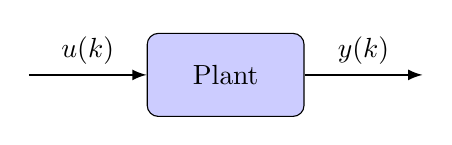
\begin{tikzpicture}[auto, node distance=2.5cm, >=latex]
    % Define styles
    \tikzstyle{block} = [rectangle, draw, fill=blue!20, 
                          text width=5em, text centered, rounded corners, minimum height=3em]
    \tikzstyle{input} = [coordinate]
    \tikzstyle{output} = [coordinate]
    \tikzstyle{arrow} = [thick,->,>=latex]
    
    % Nodes
    \node [input] (input) {};
    \node [block, right of=input] (plant) {Plant};
    \node [output, right of=plant] (output) {};
    
    % Draw arrows
    \draw [arrow] (input) -- node [above] {$u(k)$} (plant);
    \draw [arrow] (plant) -- node [above] {$y(k)$} (output);
\end{tikzpicture}\end{center}
\newpage

\subsubsection{General black-box EIV set-up}

\textit{Error-In-variables}, or EIV, problems refer to the most general case where both input and output collected samples are affected by noise, as represented in the figure \ref{fig:EIV}.\\
Two a-priori assumption is required at this point:\\
\begin{itemize}
\item a-priori assumption on the model: \(f \in F\) where \(F\) is a given class of functions
\item a-priori assumption on the noise: e.g. statistically distributed, or boundedness, etc
\end{itemize}
Then, we need to collect input-output data.
\begin{factbox}
\textbf{Without any assumption} about the noise corrupting the measurements, we cannot study the data at hand. Further, without any assumption about the structure, many structure can be find that map input samples to the output, that does not correspond to the behavior of the system. 
\end{factbox}

\begin{figure}[htbp]
    \centering
    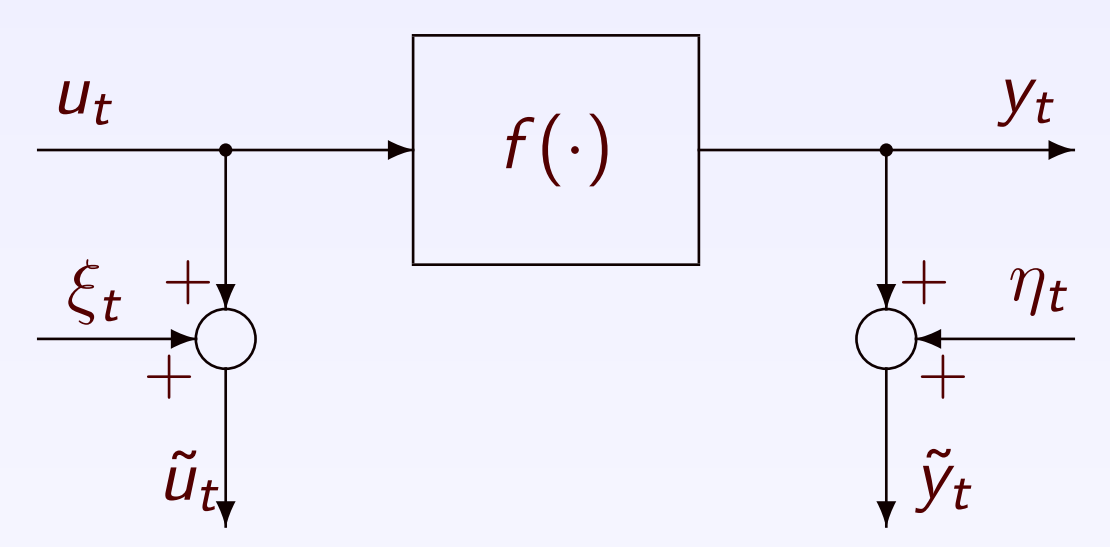
\includegraphics[width=0.5\textwidth]{images/EIV-problem.png}
    % Adjust width as needed
    \caption{a general shceme of error-in-variable problem}
    \label{fig:EIV}
\end{figure}

\subsubsection{A naive noiseless example}

Consider the following second order LTI discrete-time system (agent):

\begin{equation}
\begin{array}{l}
y(k) = f(y(k - 1), y(k - 2), u(k), u(k - 1), u(k - 2)) \\[1ex]
= -\theta_1 y(k - 1) - \theta_2 y(k - 2) + \theta_3 u(k) + \theta_4 u(k - 1) + \theta_5 u(k - 2)
\end{array}
\end{equation}

By introducing the backward shift operator \(q^{−r}\): \(q^{−r}(s(t))\)  = \(s(k − r)\), we can
rewrite the equation as:
\begin{equation}
y(k) = -\theta_1 q^{-1} y(k) - \theta_2 q^{-2} y(k) + \theta_3 u(k) + \theta_4 q^{-1} u(k) + \theta_5 q^{-2} u(k)
\end{equation}
Solving the equation in the \(y(k)\) we obtain:\\
\begin{equation}
y(k) = \frac{\theta_3 + \theta_4 q^{-1} + \theta_5 q^{-2}}{1 + \theta_1 q^{-1} + \theta_2 q^{-2}} u(k)
\end{equation}
By applying properties of the Z-transform it is possible to show that the system
transfer function G(z) can be obtained by simply replacing \(q^{-1}\) with \(z^{-1}\):
\begin{equation}
G(z) = \frac{Y(z)}{U(z)} = \frac{\theta_3 z^2 + \theta_4 z + \theta_5}{z^2 + \theta_1 z + \theta_2} u(k)
\end{equation}

Given H experimentally collected input-output samples matrix \ref{eq:regressor}, which is also called \textbf{\textit{regressor-matrix}}, leads to the following system of linear equations:
\begin{equation}
    y = A\theta
\end{equation}
where \(y = [y(3) y(4) ... y(H)]^T, \theta = [\theta_1 \theta_2 ... \theta_5]^T)\), and

\begin{equation}
    A = \left[
    \begin{matrix}
    -y(2) & -y(3) & u(3) & u(2) & u(1) \\
    -y(3) & -y(2) & u(4) & u(3) & u(2) \\
    \cdots & \cdots & \cdots & \cdots & \cdots   \\
    \cdots & \cdots & \cdots & \cdots & \cdots   \\
    -y(H-1) & -y(H-2) & u(H) & u(H-1) & u(H-2)
    \end{matrix} 
    \label{eq:regressor}
    \right]\\
\end{equation}

In this ideal, noise-free example, \(H = \text{the number of parameters} + \text{the order of the systerm}\), in this case, \(H = 7\) is enough to solve our 5-equations-and-5-unknown problem. The solution is going to be in the following form
:\\
\begin{equation}
    \theta = A^{-1} y
    \quad \overset{\text{Existence and Uniqueness Condition}}{\Rightarrow} \quad
    \begin{cases}
        
        A \in \mathbb{R}^{n \times n} \\
        \left|A\right| \neq 0
        
    \end{cases}
\end{equation}
One possible solution: apply to the system a random input sequence \(u\).\\

This formulation works for all the description that the output of the system is \textbf{linear with respect to the parameters}.

\begin{factbox}[Professor's Quote]
    In artificial-neural-network, the structure of \(f\) is different. Otherwise, the goal of any Machine Learning or System Identification problem is to find the mapping between the inputs and outputs.\\
    Regarding the importance of a-priori info about the system. The previous problem can also be solved for the following structure, that does no correspond to the behavior of a 2-order LTI system.
    \(y(k) = \theta_1 u(k) + \theta_2 u(k)^2 + \cdots + \theta_5 u(k)^5\)
\end{factbox}

\begin{example}[Example]
    It is desired to estimate the value of a resistor. A-priori info is that a resistor follows Ohm's law. As input signal, we insert current to our resistor and we measure the voltage across our resistor. \\
    
    \(y(k) = \theta u(k) \text{ s.th. y(.),u(.), }\theta \in \mathbb{R}\)\\
  
Here, \(\theta\) stands for the value of the resistor to be estimated. For this static system, which means the output of the system depends only on the values of the input at that time instance, we need a pair of noise-free input-output sample to estimate the value of the resistor. \\

\(\theta = \frac{y(1)}{u(1)}\)\\
\end{example}

\subsubsection{Noise effect}
If the measurements are corrupted by noise, the idea is to perform more measurements to average out the effect of the noise; \(H >> 2n + 1\) where n is the system order.\\

In this case, matrix\(A\) is not square anymore, which means it is not invertible. In this case, left pseudo-inverse, \((A^TA)^{-1}A^T\) of this matrix should be used.\\

\[
\tilde{y} = A \theta
\Rightarrow
A^T\tilde{y} = A^TA \theta
\Rightarrow
\theta = (A^TA)^{-1}A^T\tilde{y}
\]

This solution corresponids to the solution of the \textbf{\textit{Least Square}} problem.

\subsubsection{Least Square approach}

Least Square approach is solving the following optimization problem in order to find the parameters that minimizes a norm-2, or euclidian norm, cost-function.
\begin{equation}
    \hat{\theta_{LS}} = \arg \min \limits_{\theta} J(\theta) = \arg \min \limits_{\theta} \|\tilde{y} - A \theta\|_2
\end{equation}
In the context of system identification (but not only) θLS as what we refer to as
the Least square estimate of the system parameter vector. Computation burden of the Least square algorithms is quite low also for large H. The Least square estimate can be (also) computed recursively (i.e. online).
\newpage
\subsubsection{Consistency property of Least Square method}

If the following assumptions are satisfied:
\begin{enumerate}
\item The effect of the uncertainties corrupting the collected data can be taken into
account by introducing an additive term \textbf{e}, or equation error, as follows:
\[\tilde{y}(k) = y(k) + e(k)\]
\item  \(e(k)\), \(k = 1, 2, . . . , H\) are \textbf{independent and identically distributed} (iid) random
variables; typically it is assumed that \(e\) can be modeled as a white, zero-mean
Gaussian noise.
\end{enumerate}
Least-Square method enjoys the following interesting property:
\begin{equation}
\lim\limits_{H \to \infty} E[\theta_{LS}] = \theta
\end{equation}
Pay attention that, in our assuption, there is no argument about the variance of the noise. This is the reason why \textit{LS} method is so appealing in practice. Nevertheless, if these two assumtions does not hold, this method is not going to provide suitable results.

\begin{QandAbox}
\textbf{This property of the Least Square solution holds only when the afforementioned consistency conditions hold.\\
Every time, this method is to be applied to an engineering problem, these two assumptions should be satisfied so that the concistency property holds.
}\end{QandAbox} \vspace{0.5cm}

\textbf{As to the first assumption}, Let's check whether such an assuption is satisfied when we collect the data by performing a real experiment in its most general form, Error-In-Variable form \ref{fig:EIV}. Considering a second-order LTI system - a-priori information about the system - we have:
\[
y(k) = -\theta_1 y(k - 1) - \theta_2 y(k - 2) + \theta_3 u(k) + \theta_4 u(k - 1) + \theta_5 u(k - 2)
\]
Additionally, considering EIV form:
\[
\begin{cases}
    \tilde{y}(k) = y(k) + \eta(k)\\
    \tilde{u}(k) = u(k) + \zeta(k)
\end{cases}
\]

\begin{factbox}[Regarding the noise]
It's correct that the same sensor might be used for obtaining data samples - suggensting that the noises are dependent. Nonetheless, we assume that all the systematic error of the sensor is taken into considerations, and \textbf{\(\zeta(.)\) and \(\eta(.)\) are undeterministic noises}.\\

Also, here, an \textbf{absolute error} is considered which is the form:\\
\(\tilde{y}(.) = y(.) + \eta(.)\)
\end{factbox}
\newpage
\begin{factbox}
In case of \textbf{relative error}, the following manipulations may be done which leads to a mathematically equivalent structure.\\
\(\tilde{y}(.) = y(.)(1 + \eta(.))\)\\
Also in this case, the same result is going to be obtained.
\end{factbox}
By replacing \(y(k)\) and \(u(k)\) in the difference equation of the system the following is obtained:
\[
\begin{array}{l}
\tilde{y}(k) - \eta(k) = -\theta_1(\tilde{y}(k-1)) - \eta(k-1) -\theta_2(\tilde{y}(k-2) - \eta(k-2)) + \theta_3(\tilde{u}(k) + \xi(k)) \\[1ex] 
+ \theta_4(\tilde{u}(k-1) + \xi(k-1))
 \theta_5(\tilde{u}(k-2) + \xi(k-2)) \\[1ex] 
\Rightarrow \\[1ex]
\tilde{y}(k)= -\theta_1 \tilde{y}(k - 1) - \theta_2 \tilde{y}(k - 2) + \theta_3 \tilde{u}(k) + \theta_4 \tilde{u}(k - 1) + \theta_5 \tilde{u}(k - 2) \\[1ex]
\textcolor{red}{\fbox{\textcolor{black}{$+ \theta_1\eta(k-1) + \theta_2\eta(k-2) - \theta_3\xi(k) - \theta_4\xi(k-1) - \theta_5\xi(k-2) + \eta(k) $}}} =: + e(k) \\
\end{array}
\]
Hence:
\begin{equation}
\begin{array}{l}
\tilde{y}(k)= -\theta_1 \tilde{y}(k - 1) - \theta_2 \tilde{y}(k - 2) + \theta_3 \tilde{u}(k) + \theta_4 \tilde{u}(k - 1) + \theta_5 \tilde{u}(k - 2) + \textbf{e(k)}
\end{array}
\end{equation}

As it can be seen, considering the afformentioned assumption about noise and system, \textbf{the first assumption of the concistency property is hold!}.\\

\textbf{As to the second assumption}, it is needed to check whether the sequence \(e(k)\), \(k = 1,2, \cdots, H\) is i.i.d, independent and identically distributed. To do so, the value of \(e(k)\) is written for two time instances \(k\) and \(k+1\):
\[
\begin{array}{l}
e(k) = \theta_1\eta(k-1) + \theta_2\eta(k-2) - \theta_3\tilde{u}(k) - \theta_4\tilde{u}(k-1) - \theta_5\tilde{u}(k-2) \\[1ex]
e(k+1) = \theta_1\eta(k) + \theta_2\eta(k-1) - \theta_3\tilde{u}(k+1) - \theta_4\tilde{u}(k) - \theta_5\tilde{u}(k-1)
\end{array}
\]
As it can be seen, since both \(e(k+1)\) and \(e(k)\) depend on common variables, the sequence \(e(.)\) is not i.i.d; \textbf{the second is not satisfied}.\\

In conclusion, Least-Square estimation applied to \(\tilde{u}(.)\) and \(\tilde{y}(.)\), collected from an experiment enjoying the EIV structure provide and estimation, \(\hat{theta}_{LS}\) which does not enjoy consistency property. That is,
\[
\lim\limits_{H \to \infty} E[\theta_{LS}] \neq \theta
\]

\textbf{Results:}\\
Least-Square estimation \textbf{DOES NOT} enjoy the consistency properties when applied to input-output data obtained by performing an experiment on a dynamicsl system in the presence of an uncertainty entering the problem according to the \textit{EIV} or \textit{Output-Error} setting. 
\newpage
In which cases, assuption 1 and 2 are both satisfied?\vspace{0.5cm} \\
\(
\begin{cases}
\text{Assuption 1:}\\ 
\hspace{1cm}
\begin{array}{l}
\tilde{y}(k)= -\theta_1 \tilde{y}(k - 1) - \theta_2 \tilde{y}(k - 2) - \cdots -\tilde{y}(k - n) \\[1ex] + \theta_{n+1} \tilde{u}(k) + \theta_{n+2} \tilde{u}(k - 1) + \cdots + \theta_{n+m+1}\tilde{u}(k - m) + \textbf{e(k)}
\end{array}\\
\text{Assumption 2:}\\
\hspace{1cm}
e(.) \text{ is an i.i.d variable}
\end{cases}
\)\\

Let's consider, for the sacke of simplicity and without loss of generality, that the inputs are perfectly known.
\[
\begin{array}{l}
\tilde{u}(.) = u(.) \\ [2ex]
\tilde{y}(k)= -\theta_1 \tilde{y}(k - 1) - \theta_2 \tilde{y}(k - 2) - \cdots -\tilde{y}(k - n) \\[1ex] + \theta_{n+1} u(k) + \theta_{n+2} u(k - 1) + \cdots + \theta_{n+m+1} u(k - m) + e(k) \\[2ex]
\Rightarrow \\[2ex]
\tilde{y}\left[\theta_{n+1} + \theta_{n+2} q^{-1} + \cdots + \theta_{n+m+1} q^{-m}\right] =
= u(k)\left[1 + \theta_1 q^{-1} + \theta_2 q^{-2} + \cdots + \theta_n q^{-n}\right] + e(k)\\[2ex]
\Rightarrow \\[2ex]
\tilde{y}
= \frac{\left[1 + \theta_1 q^{-1} + \theta_2 q^{-2} + \cdots + \theta_n q^{-n}\right]}{\left[\theta_{n+1} + \theta_{n+2} q^{-1} + \cdots + \theta_{n+m+1} q^{-m}\right]}u(k) 
+ \frac{1}{\left[\theta_{n+1} + \theta_{n+2} q^{-1} + \cdots + \theta_{n+m+1} q^{-m}\right]}e(k)
\end{array}
\]
Now, considering that the equivalent of delay-operator in the \(z\)-domain is \(z\):
\[
\tilde{y} = G(z) u(z) + \frac{1}{D(z)} e(z)
\]
where,
\[
G(z) = \frac{N(z)}{D(z)} 
\begin{cases}
N(z) = \left[1 + \theta_1 q^{-1} + \theta_2 q^{-2} + \cdots + \theta_n q^{-n}\right] \\
D(z) = \left[\theta_{n+1} + \theta_{n+2} q^{-1} + \cdots + \theta_{n+m+1} q^{-m}\right]
\end{cases}
\]
The block diagram scheme of the abovementioned equation is drawn hereunder.\\
\begin{center}
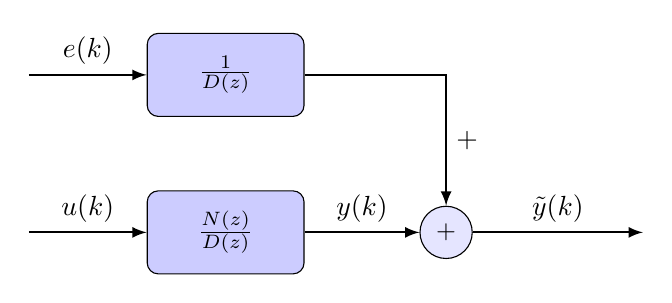
\begin{tikzpicture}[auto, node distance=2.5cm, >=latex]
    % Define styles
    \tikzstyle{block} = [rectangle, draw, fill=blue!20, 
                          text width=5em, text centered, rounded corners, minimum height=3em]
    \tikzstyle{input} = [coordinate]
    \tikzstyle{output} = [coordinate]
    \tikzstyle{sum} = [draw, fill=blue!10, circle, node distance=1.5cm]
    \tikzstyle{arrow} = [thick,->,>=latex]
    
    % Nodes
    \node [input] (input) {};
    \node [block, right of=input] (Gz) {$\frac{N(z)}{D(z)}$};
    \node [output, right of=Gz] (output) {};
    \node [block, above of=Gz, node distance=2cm] (Dz) {$\frac{1}{D(z)}$};
    \node [sum, right of=Gz, node distance=2.8cm] (sum) {\small$+$};
    \node [input, left of=Dz, node distance=2.5cm] (errorInput) {};
    \node [output, right of=sum, node distance=2.5cm] (ytilde) {};

    % Draw arrows
    \draw [arrow] (input) -- node [above] {$u(k)$} (Gz);
    \draw [arrow] (Gz) -- node [above] {$y(k)$} (sum);
    \draw [arrow] (sum) -- node [above] {$\tilde{y}(k)$} (ytilde);
    
    % Error signal and Dz block
    \draw [arrow] (errorInput) -- node [above] {$e(k)$} (Dz);
    \draw [arrow] (Dz) -| node [near end, right] {$+$} (sum);

\end{tikzpicture}
\end{center}



LS estimation is going to make sense, if and only if the sensor used for collecting data affect the collected data with a measurement noise obtained as a random, white signal \(e(k)\) that is filtered by the denominator of the system to be identified, \textbf{which does not make sense}!!!; the name of this setting is \textbf{\textit{Error-in-Equation}} setting, which does not correspond to data collection in practical situation, since the sensor does not know how to filter the noise to obtain \(e(k)\) that are probabilistically independent.\\

Our general conclusion is that Least-Square estimation should not be used when our collected via \textbf{a real experiment, EIV setting or OE setting}(OE is a subset of EIV problem, meaning that the input signal is perfectly known and the uncertainty affects output measurements dirrectly); that is, when we collect data from the experiment, even if the input is perfectly known, the output would be corrupted by additive or multiplicative noise by the data; using these data samples, LS method does not enjoy consistency property. However, Assumption 1 is satisfied and perfectly make sense when the LTI system to be identified is such that \(D(z) =  1\).\\
\[
D(z) = 1 \Rightarrow
\begin{cases}
\textcolor{red}{\fbox{\textcolor{black}{$
\text{Identification of \textbf{FIR (finite impulse response)}}
$}}}\\
\textcolor{red}{\fbox{\textcolor{black}{$\text{Identification of \textbf{static systems}}
$}}}
\end{cases}
\]
The reason is that when \(D(z) = 1\), the equation error \(e(k)\) is actually playing the role of the output measurement error \(\eta(k)\), which means i.i.d by definition, thereby satisfying also assumption 2. Now, some identification problems where both assumptions are satisfied.\\

\begin{example}[Examples that satisfies assuptions of the consistency property]
\textbf{1) A Finite-Pulse Response system} is defined in the following fashion:\\
    \(\mathbb{S}: y(k) = \theta_1 u(k) + \theta_2 u(k-1) + \cdots + \theta_n u(k-n+1)\)\\
  
Measured samples of the output have the following form:\\
\(
\begin{array}{l}
\tilde{y}(k) = y(k) + \eta(k)\\
\Rightarrow\\
\tilde{y} = \theta_1 u(k) + \theta_2 u(k-1) + \cdots + \theta_n u(k-n+1) + e(k)
\end{array}
\)\\
Where \(e(.) = \eta(.) \).\\

\textbf{2) Static Systems}: \\
\(\mathbb{S}: y(k) = f(u(k),\theta) = \theta_1 f_1(u(k)) + \theta_2 f_2(u(k)) + \cdots + \theta_n f_n(u(k))\)\\
Measured samples of the output have the following form:\\
\(
\begin{array}{l}
\tilde{y}(k) = y(k) + \eta(k)\\
\Rightarrow\\
\tilde{y} = \theta_1 f_1(u(k)) + \theta_2 f_2(u(k)) + \cdots + \theta_n f_n(u(k)) + e(k)
\end{array}
\)\\
such basis functions as polinomials or sinusoidal functions.\\
Where again, \(e(.) = \eta(.) \).\\
\end{example}
\begin{example}
Examples of functions \(f_n\) can be any set of 
In this case, the error \(e(k)\) enters the equation in an \textit{Error-in-Equation} fashion, which is required to satisfy the second assumption of the consistency property of LS.

\begin{center}
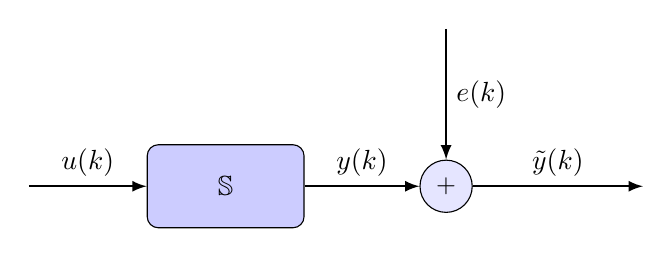
\begin{tikzpicture}[auto, node distance=2.5cm, >=latex]
    % Define styles
    \tikzstyle{block} = [rectangle, draw, fill=blue!20, 
                          text width=5em, text centered, rounded corners, minimum height=3em]
    \tikzstyle{input} = [coordinate]
    \tikzstyle{output} = [coordinate]
    \tikzstyle{sum} = [draw, fill=blue!10, circle, node distance=1.5cm]
    \tikzstyle{arrow} = [thick,->,>=latex]
    
    % Nodes
    \node [input] (input) {};
    \node [block, right of=input] (Gz) {$\mathbb{S}$};
    \node [output, right of=Gz] (output) {};
    \node [sum, right of=Gz, node distance=2.8cm] (sum) {\small$+$};
    \node [input, above of=sum, node distance=2cm] (errorInput) {};
    \node [output, right of=sum, node distance=2.5cm] (ytilde) {};

    % Draw arrows
    \draw [arrow] (input) -- node [above] {$u(k)$} (Gz);
    \draw [arrow] (Gz) -- node [above] {$y(k)$} (sum);
    \draw [arrow] (sum) -- node [above] {$\tilde{y}(k)$} (ytilde);
    
    % Error signal directly to summation point
    \draw [arrow] (errorInput) -- node [right] {$e(k)$} (sum);
\end{tikzpicture}
\end{center}
In these cases, both assumptions are satisfied, since, by assumption \(\eta\) is considered to be i.i.d, and since the error directly enters the output the first assumption is satisfied, which means:\\
\(\lim\limits_{H \to \infty} \hat{\theta}_{LS} = \theta\)\\
\end{example}

what is critical is the combination of the two assumptions, and no matter what is the structure of the system, we can always manage to define \(e(k)\) in a way that it satisfies the first assumption. The problem is that we also have to impose an additional condition, being i.i.d, on \(e(k)\) so that also the second assumption is satisfied, while based on the system equation and the way we defined \(e(k)\), this condition might not be satisfied.\\

Our next step is to reformulate this problem in a different fashion, by modifying assumption 2. In another words, it is aimed to replace assumption 2 by a "weaker assumption." This change of perspective leads to what we call \textit{Set-membership} approach to system identification.\\

\begin{QandAbox}[What about the unreachable and unobservable modes of the system?]
This is a somehow phylosophical question, which can be answered in two way:
\begin{enumerate}
\item From the practical point of view, at most engineering cases, the system that is designed does not include unobservable modes that are unstable. 
\item From a phylosophical point of view, these modes cannot be identified through input-output data collection.
\end{enumerate}
\end{QandAbox}


\chapter{Set-membership identification}    % For a new chapter (works in book and report class)

Set-membership approach is an alternative to the classical, statistical identification approach. Least-Square method is one possible example of statistical estimation algorithms in the context of estimation.\\



% ---------------------------------------------------------------------
% ---------------------------------------------------------------------
% ---------------------------------------------------------------------

% Declare appendix and set the equation counter format to (A.section.eqNumber)
\appendix
\renewcommand{\theequation}{\thesection.\arabic{equation}}
\input{chapters/Appendix}

\end{document}
